\chapter{Methodologies}
\label{chap:methods}

This chapter illustrates the methodology used to approach the development process of this work.The application is divided into three main independent instances: gesture recognition, 3D trajectory detection and drone controller. First of all, the Section \ref{sec:handgestrec} to create a \gls{dnn} model to recognize hand gestures, followed by Section \ref{sec:getdata} and \ref{sec:model} that describes the type of data used for this purpose and how they are generated. After, we will see about how orientation and camera-hand distance has been estimated in Section \ref{sec:orientationestimation} and \ref{subsec:cam-hand} to detect a 3D trajectory. Next, we focus on the drone controller in simulation and real. We conclude Section \ref{sec:pipeline} with a detailed explanation of the entire pipeline.

%pipeline
%mediapipe (poco perché già parlato tecnicamente)
%costruzione della rete neurale:
%	come devono essere i dati
%trasformazione matriciale
%algoritmo dei tre punti orientamento
%pitch
%yaw
%roll

\section{Hand Gesture Recognition}
\label{sec:handgestrec}
MediaPipe has a python implementation for their Hand Keypoints Detector. It is returning 2.5D coordinates of 20 hand landmarks as descripted in \ref{fig:handland}:

% https://towardsdatascience.com/control-dji-tello-drone-with-hand-gestures-b76bd1d4644f

\begin{figure}[H]
	\centering
	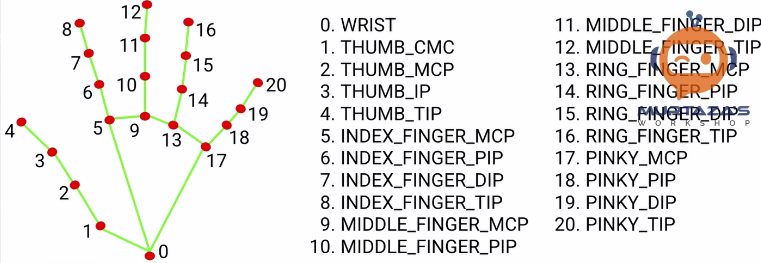
\includegraphics[width=.8\textwidth]{images/hand}
	\caption[Hand Landmarks.]{Image from the open MediaPipe repository.}
	\label{fig:handland}
\end{figure}



\subsection{Data Acquisition and Description}
\label{sec:getdata}

\subsection{Model}
\label{sec:model}

\subsection{Evaluation}
\label{sec:evaluation}

\section{3D trajectory detection}
\label{sec:3dtraj}

\subsection{Orientation estimation}
\label{sec:orientationestimation}
In the following section, we will discuss the methods used to perform yaw, roll and pitch measurements starting from the pixels of the image captured with a camera.

\subsubsection{Turning and orientations}
\label{subsec:orientationtest}
%ATTENZIONE DA FARE (citare cmsc754-spring2020-lects)
In order to find a value for the yaw we need to understand how to determine whether three points form a left-hand turn. This can be done by an orientation test, which is fundamental to many algorithms in computational geometry (citare cmsc754-spring2020-lects). Given an ordered triple of points $\langle p, q, r \rangle$ in the plane, we say that they have positive orientation if they define a counterclockwise oriented triangle (see Fig. \ref{fig:orientationtest} (a)), negative orientation if they define a clockwise oriented triangle (see Fig. \ref{fig:orientationtest} (b)), and zero orientation if they are collinear, which includes as well the case where two or more of the points are identical (see Fig. \ref{fig:orientationtest} (c)). It is important take care about the fact that the orientation depends on the order in which the points are given.

\begin{figure}[H]
	\centering
	\includegraphics[width=.8\textwidth]{images/orientationtest}
	\caption[Orientation test.]{Orientations of the ordered triple (p, q, r).}
	\label{fig:orientationtest}
\end{figure}

\noindent Orientation is formally defined as the sign of the determinant of the points given in homogeneous coordinates, that is, by prepending a 1 to each coordinate. For example, in the plane, we define:

% https://jasonwarta.github.io/latex-matrix/ 
\begin{Equation}[!htb]
	\centering
	\begin{equation}
	Orient(p,q,r) = det
	\begin{pmatrix}
	1 & p_x & p_y \\
	1 & q_x & q_y \\
	1 & r_x & r_y 
	\end{pmatrix}
	\end{equation}
	\caption[Orientation test.]{Thus orientation generalizes the familiar 1-dimensional binary relations $<, =, >$.}
	\label{eq:orientationtest}
\end{Equation}

\noindent The sign of the orientation of an ordered triple is unchanged if the points are translated, rotated, or scaled (by a positive scale factor). In general, applying any affine transformation to the point alters the sign of the orientation according to the sign of the determinant of the matrix used in the transformation. \\

\noindent If we consider points belonging to the same reference system and compute the orientation test then we can get information of how much the points are crushed together. 

\subsubsection{Yaw estimation}
\label{subsec:yaw}

\subsubsection{Roll estimation}
\label{subsec:roll}

\subsubsection{Pitch estimation}
\label{subsec:pitch}

\subsection{Camera-hand distance estimation}
\label{subsec:cam-hand}

\subsection{Univariate spline}
\label{sec:univspline}
Fitting data

\section{Drone controller}
\label{sec:dronecontrl}

\subsection{Simulation}
\label{sec:simulation}

\subsection{Real world}
\label{sec:simulation}

\section{Pipeline}
\label{sec:pipeline}
